\begin{blocksection}
\question Implement \texttt{rotate}, which takes in a tree and rotates the labels at each level of the tree by one to the left destructively. This rotation should be modular (That is, the leftmost label at a level will become the rightmost label after running rotate). You do NOT need to rotate across different branches.

For example, given the following tree,\texttt{t}

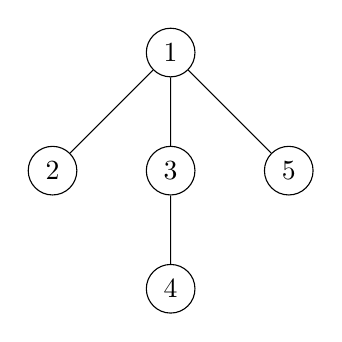
\begin{tikzpicture}[scale=1, transform shape]
\tikzstyle{level 2}=[sibling distance=10mm]
    \node [circle, draw] (z){$1$}
        child {node [circle, draw] (a) {$2$}}
        child {node [circle, draw] (d) {$3$}
            child {node [circle, draw] (g) {$4$}}
        }
        child {node [circle, draw] (b) {$5$}};
\end{tikzpicture}

calling rotate on \texttt{t} should mutate it to give us 

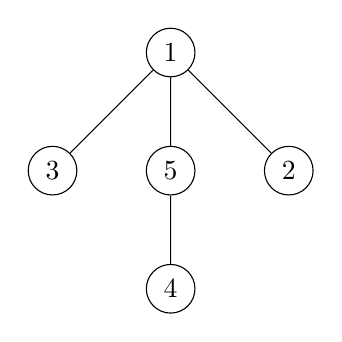
\begin{tikzpicture}[scale=1, transform shape]
\tikzstyle{level 2}=[sibling distance=10mm]
    \node [circle, draw] (z){$1$}
        child {node [circle, draw] (a) {$3$}}
        child {node [circle, draw] (d) {$5$}
            child {node [circle, draw] (g) {$4$}}
        }
        child {node [circle, draw] (b) {$2$}};
\end{tikzpicture}

\begin{lstlisting}
def rotate(t):
  """
  >>> t1 = Tree(1, [Tree(2), Tree(3, [Tree(4)]), Tree(5)])
  >>> rotate(t1)
  >>> t1
  Tree(1, [Tree(3), Tree(5, [Tree(4)]), Tree(2)])
  >>> t2 = Tree(1, [Tree(2, [Tree(3), Tree(4)]), 
                    Tree(5, [Tree(6)])])
  >>> rotate(t2)
  >>> t2
  Tree(1, [Tree(5, [Tree(4), Tree(3)]), 
                    Tree(2, [Tree(6)])])
  """
  branch_labels = ___________________________________
  n = len(t.branches)
  for ______________________________________________:
    ______________________________________________
    ______________________________________________
    ______________________________________________ 
\end{lstlisting}
\end{blocksection}

\begin{blocksection}
\begin{solution}
\begin{lstlisting}
def rotate(t):
  branch_labels = [b.label for b in t.branches]
  n = len(t.branches)
  for i in range(n):
    branch = t.branches[i]
    branch.label = branch_labels[(i + 1) % n]
    rotate(branch)
\end{lstlisting}
\end{solution}
\end{blocksection}